\chapter{Implementation} \label{implementation}

For this project I decided to use the Rust programming language. I chose
it because it makes performant, memory safe code much easier to write than
alternative systems languages such as C++ or C. Additionally, it has very good
parallel programming facilities and an extensive software ecosystem.

\begin{listing}[H]
\begin{minted}[linenos]{text}
fn factorial[n: int] {
    if n == 0 {
        return 1;
    } 

    return (n * factorial(n - 1));
}
\end{minted}
\caption{Factorial in the test language.}
\label{lst:example}
\end{listing}

\begin{listing}[H]
\begin{minted}[linenos]{json}
{
  "a": 100,
  "b": {
    "x": [
      100,
      "a"
    ]
  }
}
\end{minted}
\caption{Example of parsable JSON.}
\hrulefill
\label{lst:example}
\end{listing}

Section \ref{dependancies}
\newline \newline
Section \ref{structure}
\newline \newline
Section \ref{outputs_and_visualizations}
\newline \newline
Section \ref{debugging}

\section{Dependencies} \label{dependancies}
\section{Structure} \label{structure}
\subsection{Parsing Grammar Transformation} \label{parsing_grammar_transformation}
\section{Outputs and Visualizations} \label{outputs_and_visualizations}

\begin{figure}[t]
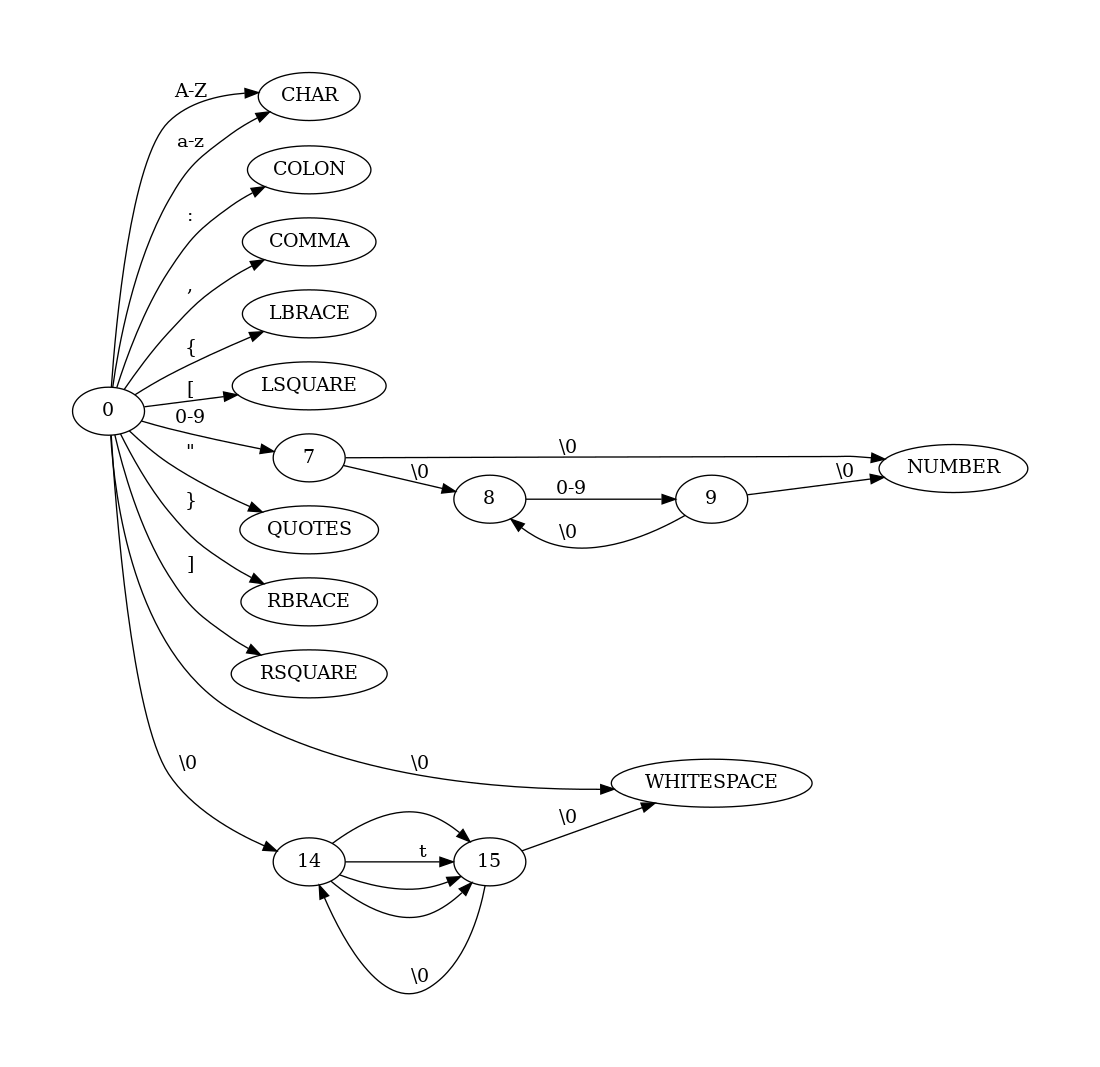
\includegraphics[width=\linewidth]{images/nfa.png}
\caption{NFA of the lexical grammar}
\label{fig:compiler}
\end{figure}

\begin{figure}[t]
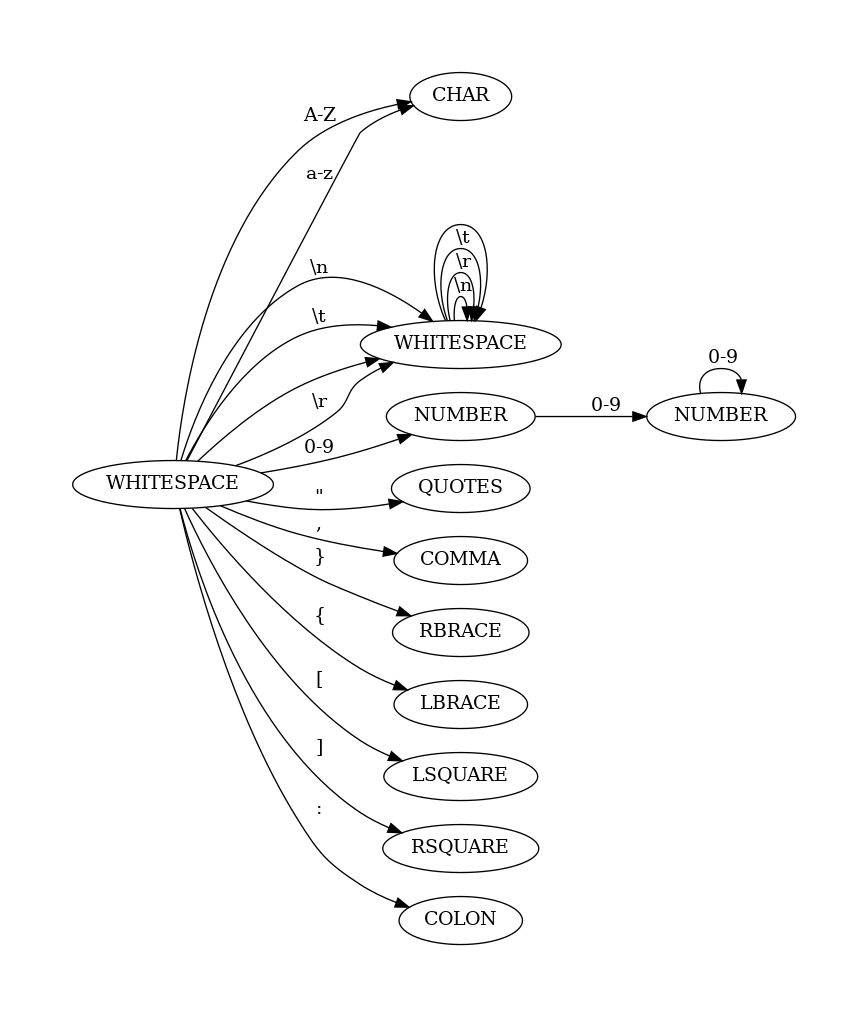
\includegraphics[width=\linewidth]{images/dfa.png}
\caption{DFA of the lexical grammar}
\label{fig:compiler}
\end{figure}

\begin{figure}[t]
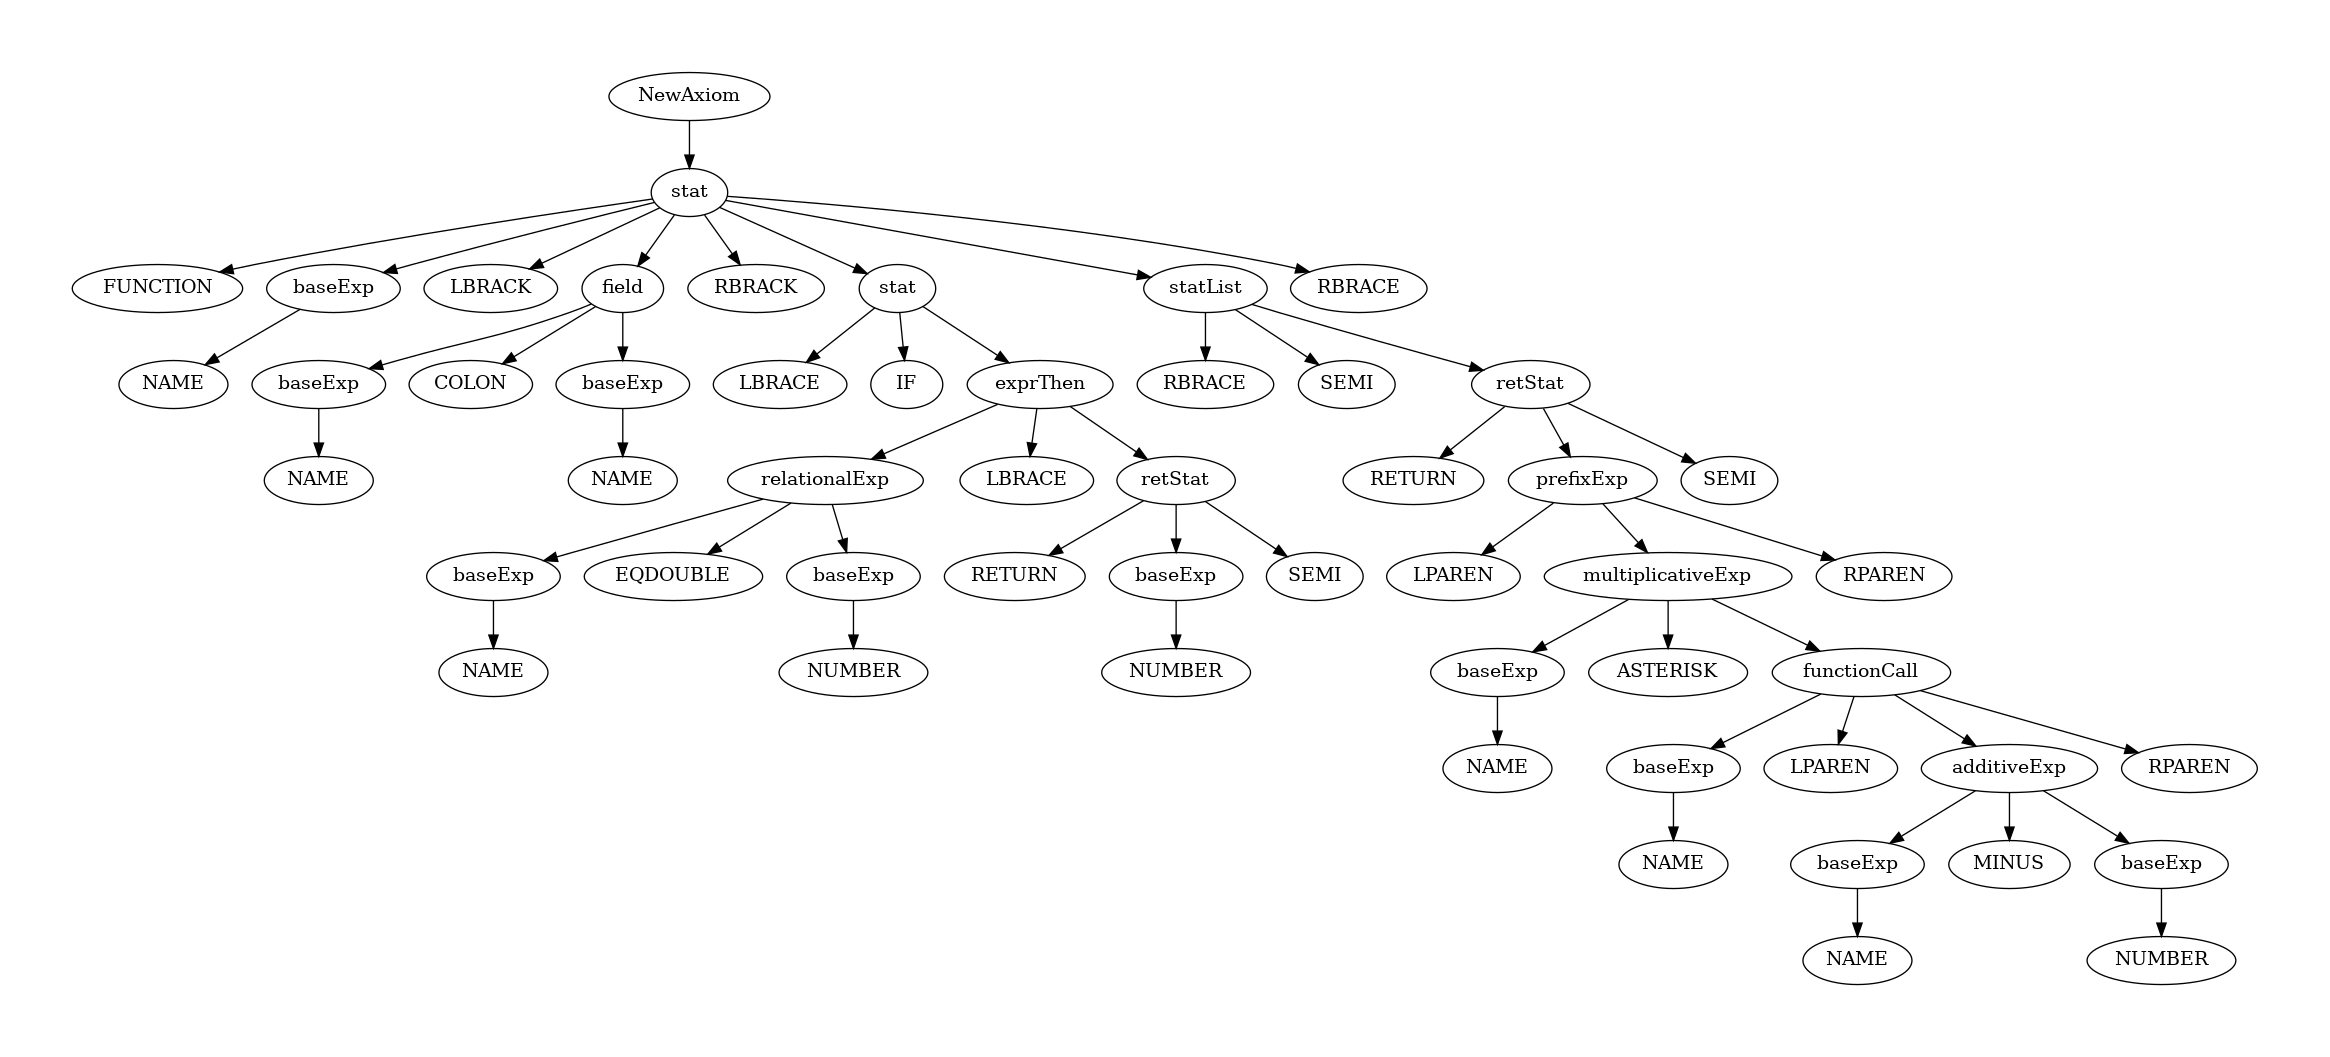
\includegraphics[width=\linewidth]{images/ptree.png}
\caption{Graphviz visualization of the parse tree.}
\label{fig:compiler}
\end{figure}

\section{Debugging} \label{debugging}
